\documentclass[11pt, a4paper, USenglish]{article} % change ``USenglish'' to ``norsk'' if applicable.

\usepackage{kyblab} % Contains all included packages. See kyblab.sty.
\usepackage{float} % Contains all included packages. See kyblab.sty.
\usepackage{mathtools}
\usepackage{pdfpages}
\addbibresource{bibliography.bib} % Makes the bibliography file available to biblatex.
\setcounter{MaxMatrixCols}{20}
\lstset{
%frame=single,
breaklines=true,
prebreak=...
}

\begin{document}

% Titlepage
\title{Lab Report TTK4135}
\author{Group 16\\Student 93841\\Student 32187}
\date{April 5, 2017}
\begin{titlepage}
    \maketitle
    \begin{figure}
    \centering
    
\includegraphics[width=0.5\textwidth]{figures/itk_ntnu}\\
    Department of Engineering Cybernetics
    \end{figure}
    \thispagestyle{empty}
\end{titlepage}

% Abstract
\newpage
\begin{abstract}
\addcontentsline{toc}{section}{Abstract} % add this if you want the abstract in the table of contents.
% This document outlines a few important aspects of a lab report. It contains some advice on both content and layout. The \LaTeX{} source for this document is also published, and you can use it as a template of sorts for your own report. You can find an up to date version of the source at \url{https://github.com/ntnu-itk/labreport}. The main file, ``labreport.tex'', defines the structure of the document. The ``preamble.tex'' file is the document preamble, and contains a lot of informative comments. The document is based on work done by Tor Aksel Heirung for TTK4135.

% When you write your own report, this section (the abstract) should contain a \emph{very} short summary of what the lab is about and what you have done.
Investigate the implementation of optimal controllers using linear quadratic regulators, SQP, and compare open and closed-loop control for a linear system using linear and nonlinear constraints.
\end{abstract}

\thispagestyle{empty} % Avoid page numbering on the abstract page.

% TOC
\newpage
\tableofcontents
\thispagestyle{empty} % Avoid page numbering on the table of contents.

% Main content
\newpage
\setcounter{page}{1}
\section{Introduction}\label{sec:intro}
Your introduction should contain an overview of the work you were assigned, as well as a few sentences putting the work into a larger perspective. You should also give a quick description of how the report is organized (as is done below).

You should of course put most of the work into doing good work in the lab and then presenting it in the report. When presenting your work in the report, both content and presentation/layout matters. Since your only way of communicating your good effort in the lab is through writing about it here, the way you write about it is essential. This means that even if you have the very best controller but describe it poorly, you will probably not be rewarded for the good results. A plot showing perfect control is worth very little if it is not accompanied by a clear description of what it represents.

Layout is naturally less important than content, but it still matters. You can think of report writing like selling an apartment; when you present your apartment for potential buyers you will of course clean the apartment and make it good looking. How clean the apartment is does of course not determine its value, but it is still important since it influences the subjective value your buyers will put on the apartment. 

\subsection{Software}
You are of course free to use whatever software you want for report writing. You can also submit a handwritten report, although this is probably not a great idea if your handwriting can be hard to read. 

You can also use Word or a similar word processor. However, it is next to impossible to achieve decent layout with Word. The support for vector graphics (discussed later) is extremely poor, and text tends to look pretty bad (bad support for kerning and ligatures). Furthermore, math is both time consuming and difficult to input, and tends to look very ugly. In general, a report written in Word looks like a draft.

It is strongly recommended to use Latex. Unless you tweak the layout too much, your report will almost certainly look very good. Although it can take a bit of effort to get started, it is also much quicker to use than Word and similar programs. The support for math and vector graphics is also great.

If you are new to Latex, you can have a look at the source for this document to get started. You can also look at the presentation by~\cite{Berland2010} (in Norwegian) or consult~\cite{Oetiker2011}. Another good reason to learn Latex is that you probably don't want to write your master's thesis in something like Word, doing so would likely be very frustrating. Being reasonably fluent in Latex before you get that far will make your thesis work much smoother.

Some of you are probably fluent in Latex and might plan to write the report using it. Please resist the temptation (if any) to change the fonts, make super fancy headers (they are not necessary for a report like this), change the margins, change the paragraph indentation and/or spacing, and similar things.

A great tool for collaborating on Latex documents is ShareLaTeX at \url{https://www.sharelatex.com/}; if you use this you won't have to install anything on your computer. Texmaker at \url{http://www.xm1math.net/texmaker/} is a good cross-platform editor. Some people like Lyx, which is a Latex editor that behaves a little bit like Word. If you prefer to compile your Latex document on the command line, the latexmk \url{https://www.ctan.org/pkg/latexmk} command is a great tool included in most TeX distributions. There is also a simple Vim plugin that uses latexmk as its backend called LaTeX-BoX \url{https://github.com/LaTeX-Box-Team/LaTeX-Box}.

\subsection{Other Comments}
Unless you have a very good reason not to, you should write the report in English. If you have problems with Latex, the solution is usually just a few Google searches away.

This report is organized as follows: \Cref{sec:prob_descr} contains some equations relevant for TTK4135, and some tips on how to create illustrations. Several \LaTeX{} tips can be foundin \Cref{sec:latex_tips}, such as how to create a table and matrix equations. \Cref{sec:figures} contains some advice on using plots from MATLAB\@. The closing remarks are in~\Cref{sec:conclusion}, respectively. \Cref{sec:matlab} contains a MATLAB file while \Cref{sec:simulink} shows an example Simulink diagram. The Bibliography can be found at the end, on page~\pageref{sec:bibliography}.

\section{Problem Description}\label{sec:prob_descr}
A cantilevered unbalanced helicopter needs to be balanced using optimizing control.
The model of the helicopter is outlined in equation.
\begin{gather}
	\ddot{e} + K_{3} K_{ed} \dot{e} + K_{3} K_{ep} e = K_{3} K_{ep} e_{c} \label{eq:model_elev} \\
	\ddot{p} + K_{1} K_{pd} \dot{p} + K_{1} K_{pp} p = K_{1} K_{pp} p_{c} \label{eq:model_pitch} \\
	\dot{\lambda} = r \label{eq:model_lambda} \\
	\dot{r} = -K_{2} p \label{eq:model_r}
\end{gather}
We can number them like this:
\begin{subequations}\label{eq:model}
	\begin{gather}
		\ddot{e} + K_{3} K_{ed} \dot{e} + K_{3} K_{ep} e = K_{3} K_{ep} e_{c} \label{eq:model_se_elev} \\
		\ddot{p} + K_{1} K_{pd} \dot{p} + K_{1} K_{pp} p = K_{1} K_{pp} p_{c} \label{eq:model_se_pitch} \\
		\dot{\lambda} = r \label{eq:model_se_lambda} \\
		\dot{r} = -K_{2} p \label{eq:model_se_r}
	\end{gather}
\end{subequations}
You can then both reference individual equations (``the elevation equation \Cref{eq:model_se_elev}'') or reference the entire model (``the linear model~\Cref{eq:model}''). Regardless of your choice of software, never hard-code a reference, always use dynamic references.

You could also align the equations like this:
\begin{subequations}\label{eq:model_al}
	\begin{align}
		\ddot{e} + K_{3} K_{ed} \dot{e} + K_{3} K_{ep} e &= K_{3} K_{ep} e_{c} \label{eq:model_se_al_elev} \\
		\ddot{p} + K_{1} K_{pd} \dot{p} + K_{1} K_{pp} p &= K_{1} K_{pp} p_{c} \label{eq:model_se_al_pitch} \\
		\dot{\lambda} &= r \label{eq:model_se_al_lambda} \\
		\dot{r} &= -K_{2} p \label{eq:model_se_al_r}
	\end{align}
\end{subequations}
You can consult~\cite{Downes2002} for more about writing math.

\subsection{Illustrations}
% If you decide to include an illustration, that's great. You can in general copy figures and illustrations from the textbook, the assignement text, or other places. However: ALWAYS CITE THE SOURCE\@. You can also draw your own (cite the source if it is heavily based on someone else's.). \Cref{fig:layers_openloop} was created quickly with Ipe (\url{http://ipe.otfried.org/}). Inkscape is a good alternative for more advanced illustrations. Some people prefer the Latex package TikZ (\url{http://texample.net/tikz/examples/}), but this takes a little effort to learn.
The following picture describes the lab setup.

% \begin{figure}[tp]
% 	\centering
% 	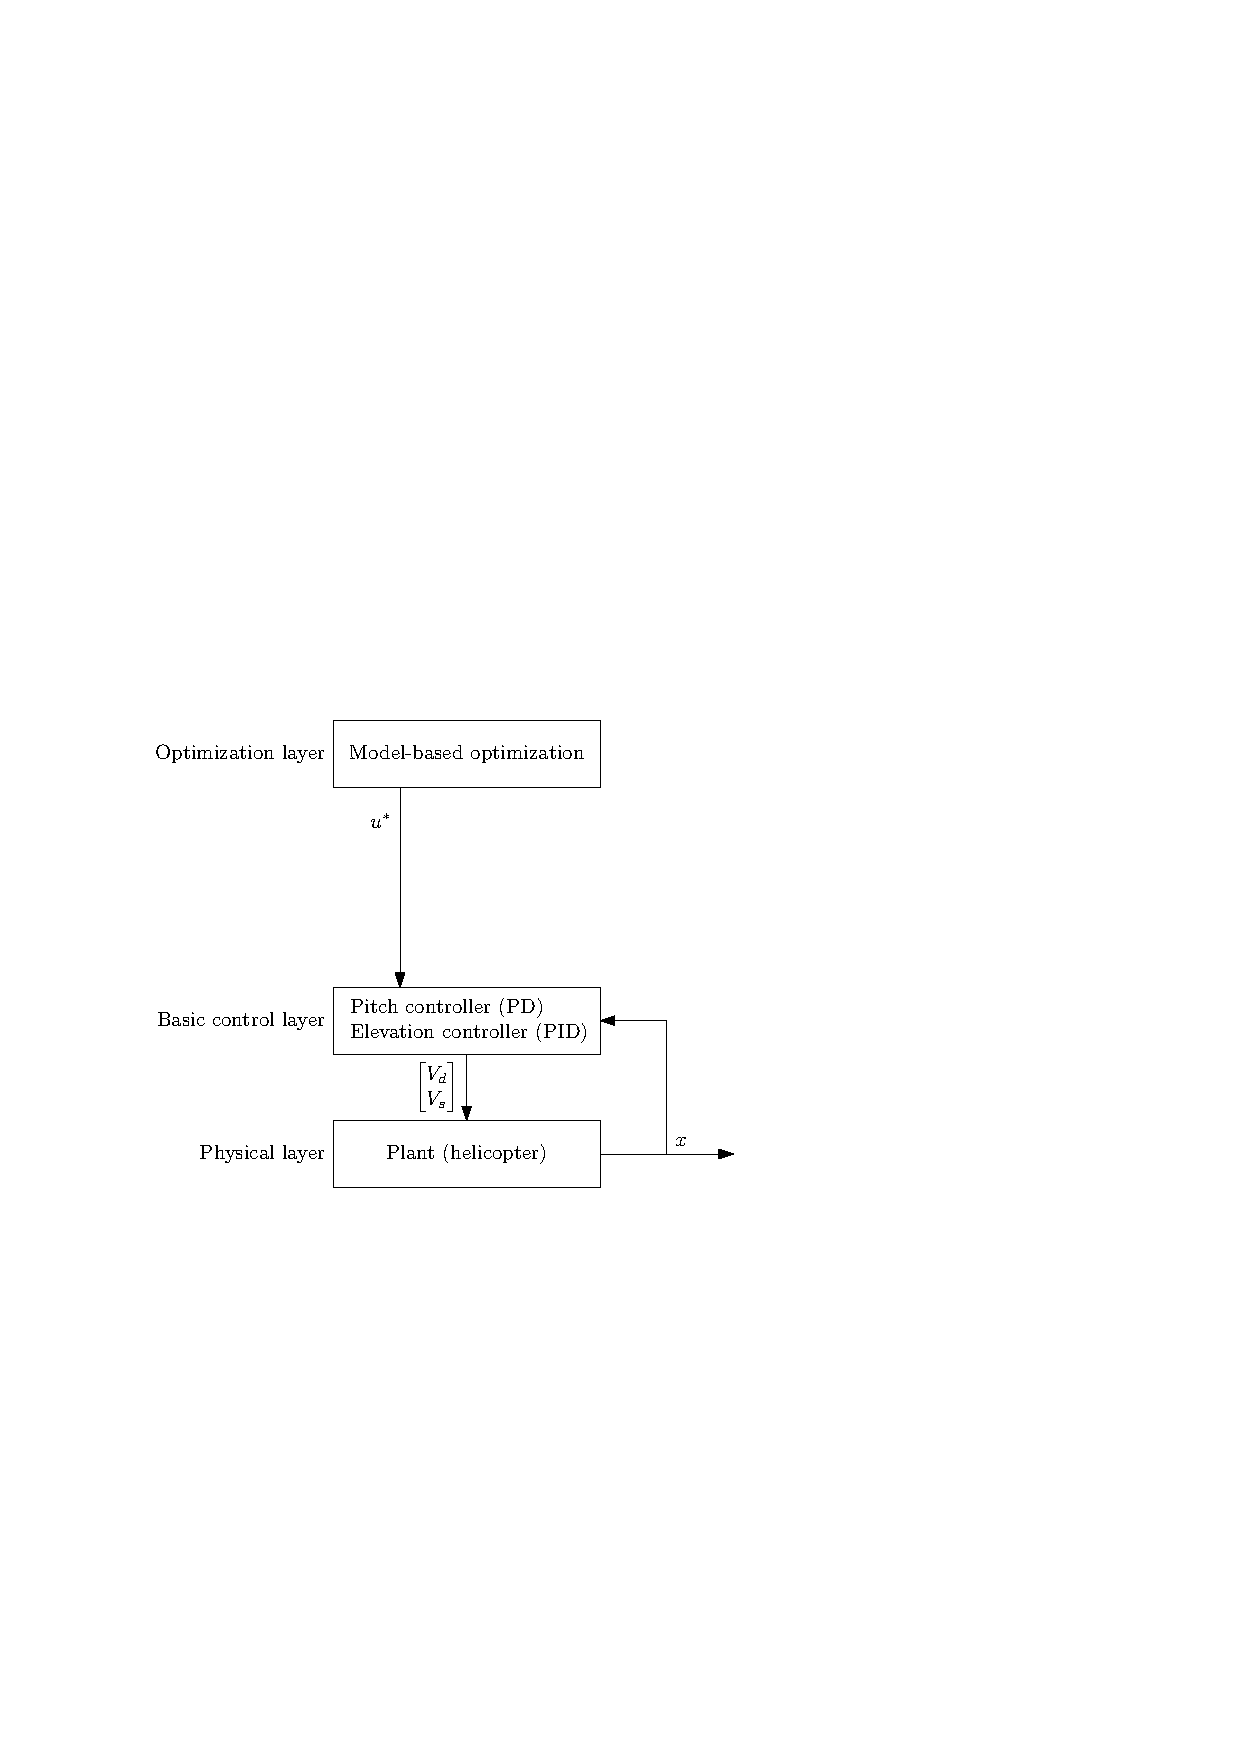
\includegraphics[width=1.00\textwidth]{figures/layers_openloop.pdf}
% 	\caption{A figure created with Ipe for TTK4135.}
% \label{fig:layers_openloop}
% \end{figure}

\newcommand{\texMacro}[2]{\texttt{\textbackslash{#1}\{#2\}}}
% \section{General LaTeX tips}\label{sec:latex_tips}
% Some tips were given in \Cref{sec:intro}, and this section will elaborate with some more concrete examples.
\section{Results and Discussion}
\subsection{Optimal Control of Pitch/Travel without Feedback}

\subsubsection{Continuous State Space Form}
% Write the model on continuous time state space form
First we must formulate the model \Cref{eq:model} in a continuous state-space form. Elevation is neglected here.

The equation for elevation \Cref{eq:model_se_elev} is completely removed from the model \Cref{eq:model} and we are left with the following set of equations.

\begin{subequations}
	\begin{align}
		\ddot{p} = - K_1K_{pd}\dot{p} - K_1K_{pp}p + K_1K_{pp}p_c \\
		\dot{\lambda} = r \\
		\dot{r} = -K_2p
	\end{align}
\end{subequations}

Since $ x = [\lambda\ r\ p\ \dot{p}]^T $, and $ u = p_c $ we can formulate $\ddot{p}$ as a vector product.

\begin{equation}
	\ddot{p} = [0\ 0\ -K_1K_{pp}\ -K_1K_{pd}] x + K_1K_{pp}\ u
\end{equation}

The change in $ p $ as:

\begin{equation}
\dot{p} = [0\ 0\ 0\ 1] x + 0\ u
\end{equation}

likewise for $ r $:
\begin{equation}
	\dot{r} = [0\ 0\ -K_2\ 0] x + 0\ u
\end{equation}
and finally $\lambda$:
\begin{equation}
	\dot{\lambda} = [0\ 1\ 0\ 0] x + 0\ u
\end{equation}

Using the formulas that were given we construct a state-space model of form in \Cref{eq:state-space}.
\begin{equation}\label{eq:state-space}
	\dot{x} = A_c\ x + B_c\ u
\end{equation}

\begin{subequations}
\begin{align}
\alpha_1 \vcentcolon= K_1K_{pp} \\
\alpha_2 \vcentcolon= K_1K_{pd} \\
A_c =
\begin{bmatrix}
    0 & 1 & 0 & 0 \\
    0 & 0 & -K_2 & 0 \\
    0 & 0 & 0 & 1 \\
    0 & 0 & -\alpha_1 & - \alpha_2
\end{bmatrix}
\label{eq:initial_state}
\end{align}
\end{subequations}

\begin{equation}
B_c =
\begin{bmatrix}
	0 \\
	0 \\
	0 \\
	\alpha_1
\end{bmatrix}
\end{equation}

% What are we modeling here? Is it just the helicopter? Discuss what the model includes, and how it relates to Figure 7.
The aforementioned model various states of the helicopter; including pitch, distance traveled, travel speed, and the input and its effects on these variables. Additionally we make the  simplifying assumptions that the pitch angle is small, and that there is no friction or air resistance acting on the helicopter resisting the direction of travel. Figure 7 in \Cref{sec:ex} contains the precomputed $u*$ which are fed into the system, which is how the model is related to the figure.

\subsubsection{Forward Euler Discretization}
% Discretize the model using the forward Euler method and write the resulting model on discrete time state space form

Using Euler's time discretization on the system's standard form we will get the following expression:

\begin{equation}
	x_{k+1} = A\ x_k + B\ u_k
\end{equation}
First we discretize the derivative vector
\begin{subequations}
\begin{align}
{\dot{x}} = \lim_{h\rightarrow 0} \frac{{x}_{k+1}-{x}_{k}}{h} \\
\Rightarrow {\dot{x}} = \lim_{h\rightarrow 0} \frac{{x}_{k+1}-{x}_{k}}{h} = {A_c} {x}_k + {B_c} u_k
\end{align}
\end{subequations}
We ignore the limit, it's implicit for $ h $.
\begin{equation}
\Rightarrow {x}_{k+1} = {x}_{k} + h({A_c} {x}_k + {B_c} u_k)
\end{equation}
Now $ {x}_k $ can be algebraically merged into a matrix.
\begin{subequations}
\begin{align}
\Rightarrow {x}_{k+1} = h{A_c} {x}_k + {x}_{k} + h{B_c} u_k \\
\Rightarrow {x}_{k+1} = (h{A_c} {I} + {I}){x}_k + h{B_c} u_k
\end{align}
\end{subequations}
This is the same as adding $ 1 $ to each diagonal in $ h{A_c} $. We rename ($hA_c{I} + {I}$) to $ {A}$ and ($h{B_c}$) to $B$.
\begin{equation} \label{mat:eq}
\Rightarrow {x}_{k+1} = {A}\ {x}_k + {B}\ u_k
\end{equation}
Where
\begin{equation}
{A} = h\ {A_c} + {I}
\end{equation}
\begin{equation}
{B} = h{B_c}
\end{equation}

This defines the discrete time state space form.


\subsubsection{Calculate an Optimal Trajectory}
%  Calculate an optimal trajectory for moving the helicopter from x 0 = λ 0 0 0 0 to x f = λ f 0 0 0 when the elevation angle is assumed to be constant. Use λ 0 = π and λ f = 0. Also implement the constraint 30π |p k | ≤ , k ∈ {1, . . . , N } [14] 180 Since the manipulated variable p c in this case is the setpoint for the p controller, the constraint should also be implemented for the manipu- lated variable. We want to minimize the cost function N [λ i − λ f ] 2 + qp 2 ci , φ = q ≥ 0 [15] i=1 Solve the optimization problem using the MATLAB function quad- prog. Try using the values 0.1, 1, and 10 as weights q. Plot the manipulated variable and the output. Comment the results with re- spect to the different weights chosen. Remember that some useful files are posted on Blackboard. Use a sampling time of 0.25 s and N = 100.  15Furthermore, discuss the objective function [15], in particular the term [λ i − λ f ] 2 . For instance, could any unwanted effects arise from steer- ing the helicopter to λ = λ f with this objective function?
We encode the equality constraint using \Cref{mat:eq}, this gives us a constraint where we have a matrix of the form
\begin{equation}
A_{eq} =
\begin{bmatrix}
    I      & 0  & 0 & 0 & \hdots & 0      & 0  & -B & 0  & 0  & \hdots & 0\\
    -A     & I  & 0 & 0 &        & 0      & 0  & 0  & -B & 0  &        & 0\\
    0      & -A & I & 0 &        & 0      & 0  & 0  & 0  & -B &        & 0\\
    \vdots &    &   &   & \ddots & \vdots & 0  &    &    &    & \ddots & \vdots\\
    0      & 0  & 0 & 0 & \hdots & -A     & I  & 0  & 0  & 0  & \hdots & -B\\
\end{bmatrix}
\end{equation}

With the constraint
\begin{equation}
{A}_{eq}^{[400x500]} {x} = {B}_{eq}
\end{equation}
Where
\begin{equation}
{B}_{eq}[t] = {0}\ \forall t > 1
\end{equation}
\begin{equation}
{B}_{eq}[1] = Ax_0
\end{equation}

The following plots convey our theoretical and practical results:

The graphs with the circles are theoretical and the one with only blue line graphs are practical. There are significant differences between these.

One can observe that setting $ q = 0.1 $ does not particularly affect travel rate in practice, but setting $ q = 10 $ affects travel rate significantly.

The objective function can be collapsed into:

$$ \sum_{i=1}^N \lambda_i^2 + qp_{ci}^2 $$

% Furthermore, discuss the objective function [15], in particular the term [λ i − λ f ] 2 . For instance, could any unwanted effects arise from steer- ing the helicopter to λ = λ f with this objective function?

when $ \lambda_f = 0 $. This term is not scaled (except for unit scaling) such that we can fully control the objective function by exploiting $ q $. An unwanted effect could be overshoot, since a high $ q $ implies $ p_{ci} $ taking priority over $ \lambda_i $.

\begin{figure}[H]
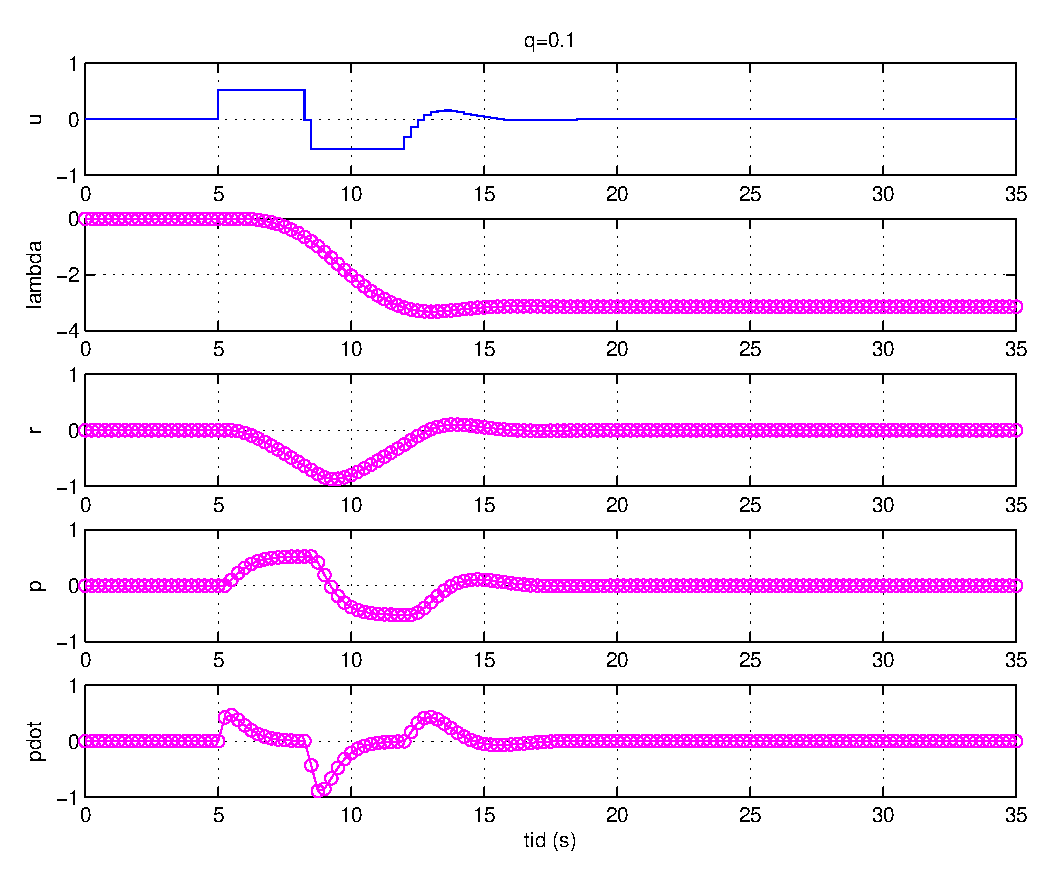
\includegraphics[scale=0.8]{{figures/10.2.3.q_0.1.theory}.eps}
\caption{Theoretical rates from the physical helicopter (q = 0.1)}
\label{fig:10.2.3.q_0.1.theory}
\end{figure}

\begin{figure}[H]
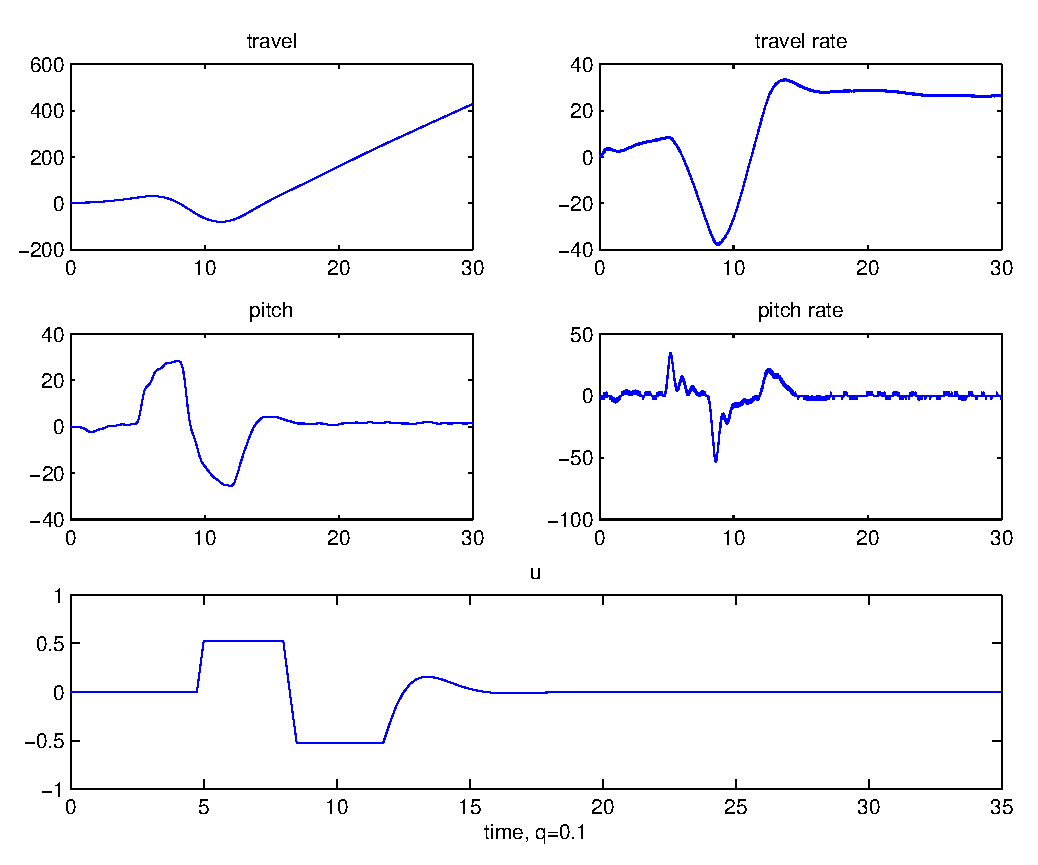
\includegraphics[scale=0.8]{{figures/10.2.3.q_0.1}.eps}
\caption{Actual rates from the physical helicopter (q = 0.1)}
\label{fig:10.2.3.q_0.1}
\end{figure}


\begin{figure}[H]
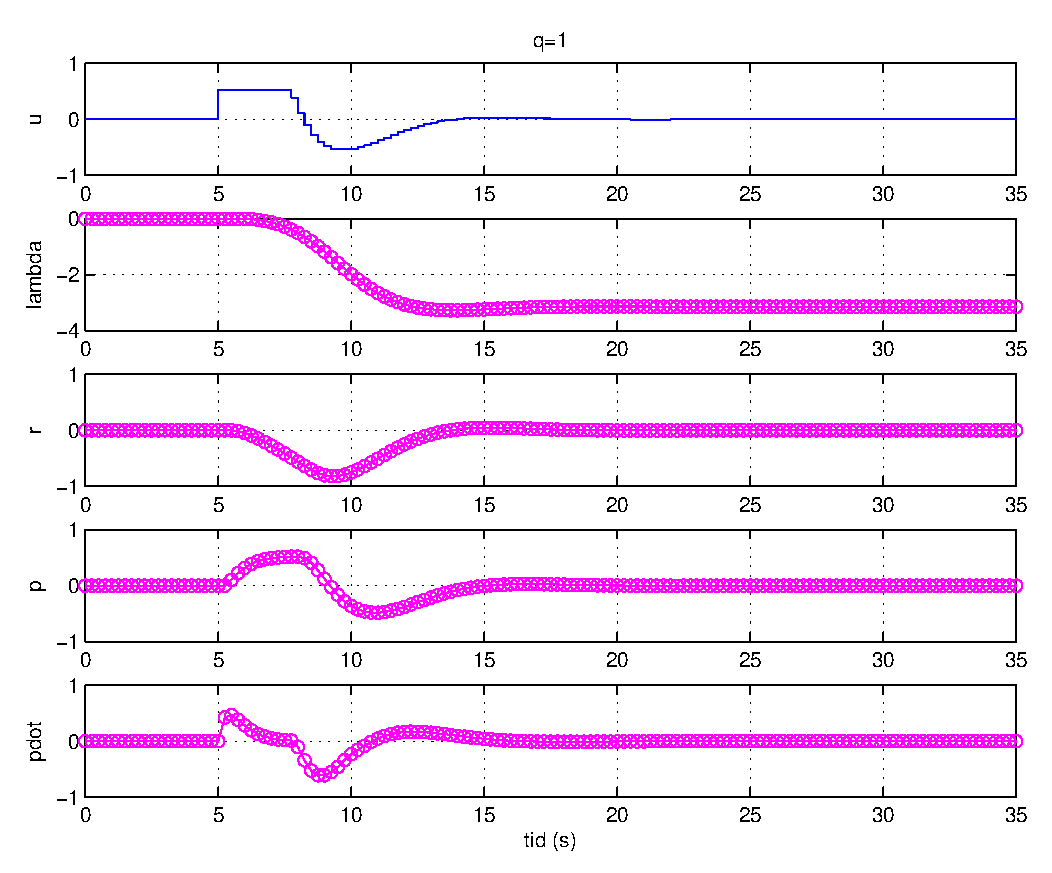
\includegraphics[scale=0.8]{{figures/10.2.3.q_1.theory}.eps}
\caption{Theoretical rates from the physical helicopter (q = 1)}
\label{fig:10.2.3.q_10.theory}
\end{figure}

\begin{figure}[H]
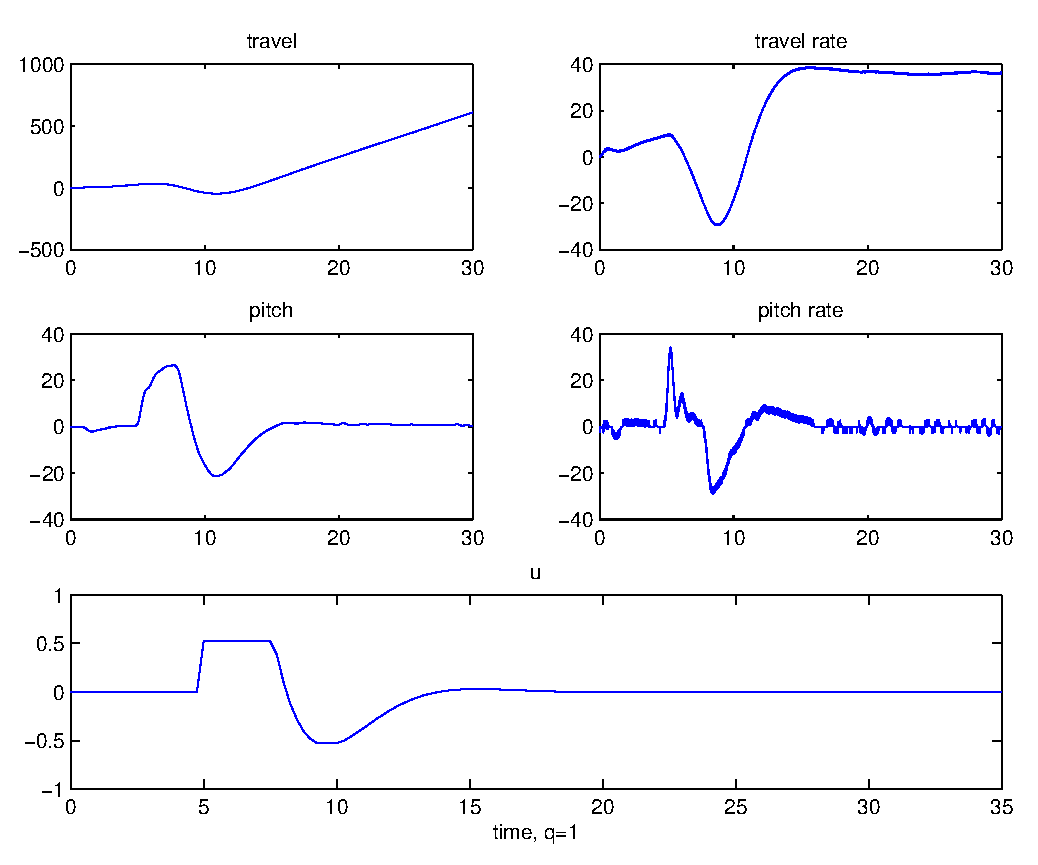
\includegraphics[scale=0.8]{{figures/10.2.3.q_1}.eps}
\caption{Actual rates from the physical helicopter (q = 1)}
\label{fig:10.2.3.q_1}
\end{figure}


\begin{figure}[H]
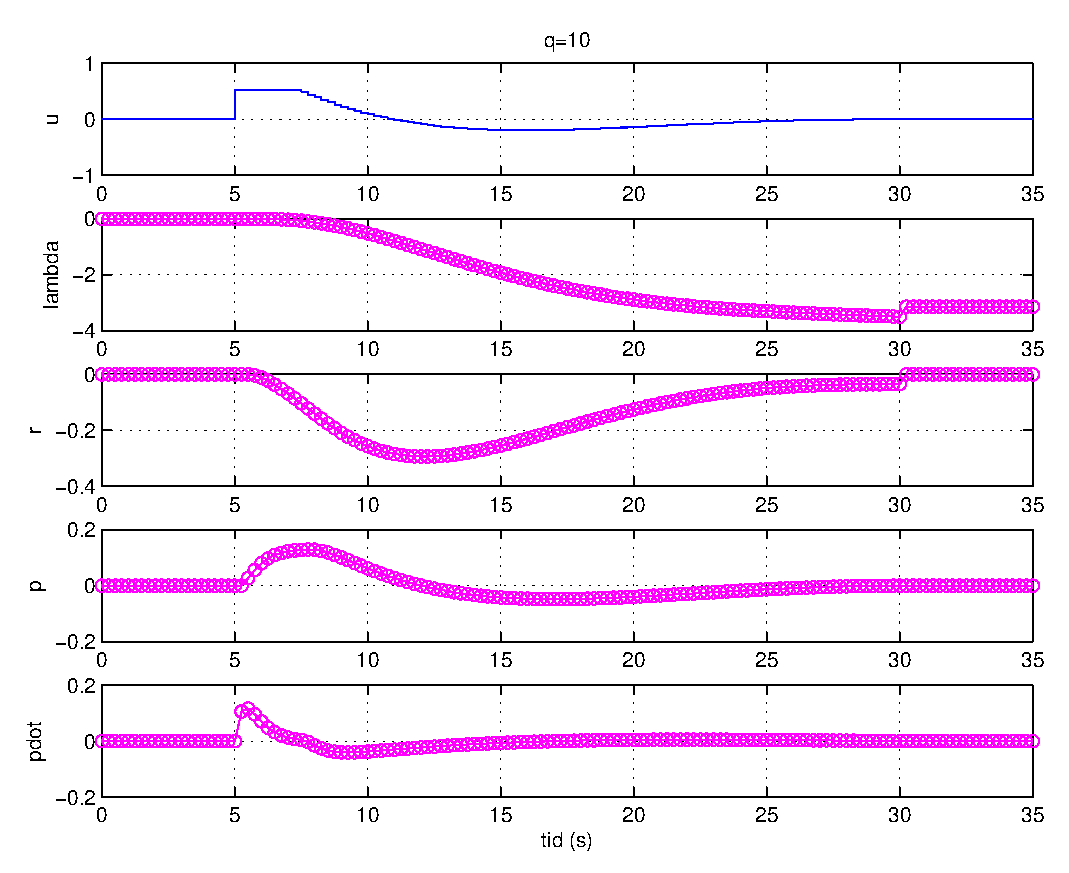
\includegraphics[scale=0.8]{{figures/10.2.3.q_10.theory}.eps}
\caption{Theoretical rates from the physical helicopter (q = 10)}
\label{fig:10.2.3.q_10.theory}
\end{figure}

\begin{figure}[H]
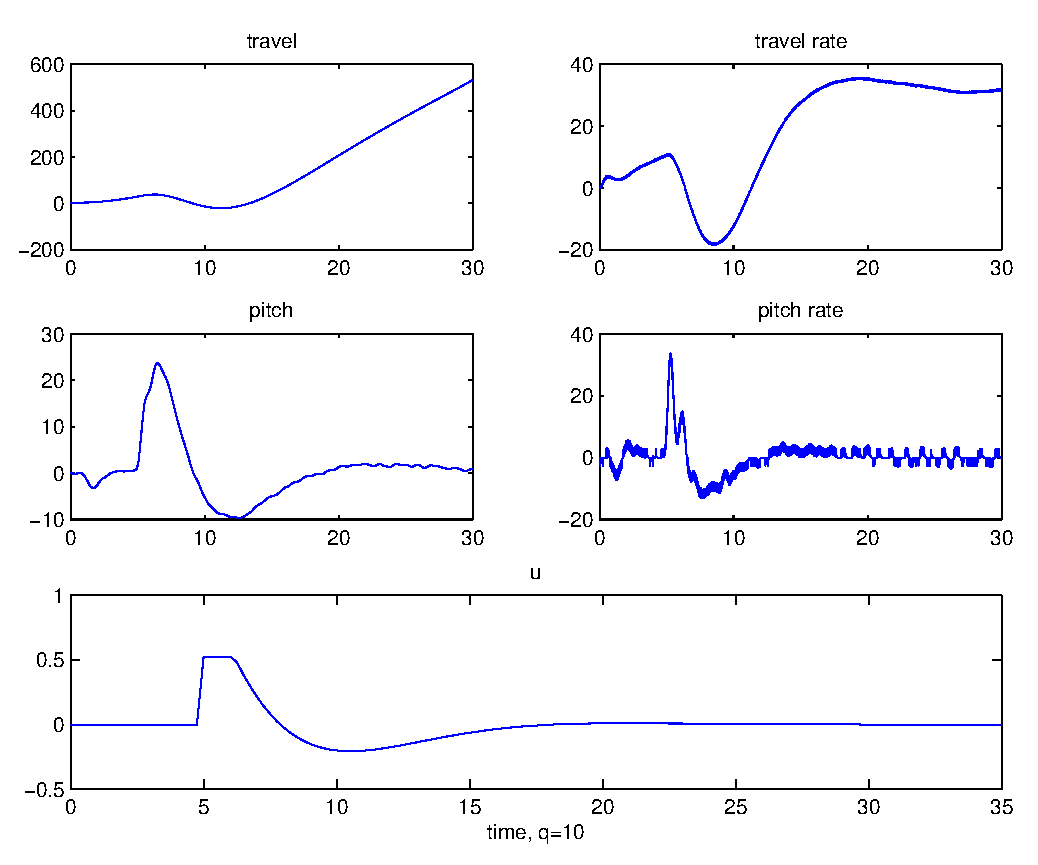
\includegraphics[scale=0.8]{{figures/10.2.3.q_10}.eps}
\caption{Actual rates from the physical helicopter (q = 10)}
\label{fig:10.2.3.q_10}
\end{figure}

\subsubsection{Offset}
% The specific implementation of the QP algorithm used here can only weight deviations from origin [λ f = 0]. The position sensors on the helicopter are relative, which means that the position is reset to zero each time the helicopter is started. To get the helicopter to start in x 0 you have to add a suitable value to the measurement. For example, you can subtract 30 ◦ from the elevation measurement to get the helicopter to fly at a reasonable height when e c = 0 [this is done in the given file]. Implement the input sequence generated in c] with q = 1.  The optimization in c] gives the manipulated variable u. It may be a good idea to add some zeros at the beginning of the input vector, so that the helicopter has time to stabilize in x 0 before the calculated sequence is implemented. Also, adding zeros at the end of the vector is recommended to keep the helicopter stable after the input sequence is over. Add enough zeros to keep the helicopter stable for at least 5 s before and after the optimal input sequence is implemented. The easiest way to transfer the input sequence to Simulink is to use a “From Workspace” block [which can be found under “Sources” in the Library Browser]. This block imports two vectors, a vector u which is connected to the output and a time vector t which determines when the different elements of u should be transfered to the output.  Does the helicopter end in the desired point x f ? What causes the observed deviation?

Implementing this optimal control sequence on the test helicopters and yielded noticable deviation from the desired final position. This is due to lack of feedback to account for physical disturbances, modeling inconsistencies and linearizion errors.

% Does the helicopter end in the desired point x f ? What causes the observed deviation?
The helicopter does not end in the desired point because there's significant clockwise bias when the helicopter is left with a zero input.

\subsection{Optimal Control of Pitch/Travel with Feedback (LQ)}

\subsubsection{LQ Control}
% In MATLAB you can use the function dlqr to calculate the optimal K matrix. Q and R indicates how much you want to penalize deviation in the states, and how much you want to penalize use of the manipulated variable. Use diagonal matrices for Q and R. A diagonal matrix is easily made in MATLAB using the function diag.
Feedback $k$ is computed using \Cref{lst:compute_lq}.  This script uses $A1$ and $B1$ which are defined in \Cref{lst:problem_2}.

\subsubsection{Simulink Feedback}
% Implement the feedback on the helicopter and run the helicopter. This is done in Simulink using the following blocks Mux, Demux, Matrix 17Multiplication, Sum, and “From Workspace”. Notice that the “From Workspace” block can import several values [a vector], meaning only one block is required for x.

\Cref{fig:feedback-3} shows the final model required for part 10.2.


\subsubsection{MPC Controller}
% An alternative strategy would be to use an MPC controller. How would you realize this controller?
We would realize the MPC controller by creating a matlab function block in the simulink diagram that uses the current state as an initial state in the horizon. After solving the horizon for $u$, we supply the first element of $u$ to as input.

% Discuss advantages and disadvantages with and MPC controller compared to the controller you have implemented.
The MPC controller may be significantly more expensive. The LQR is much simpler in that it takes one big computation on that generates a multiplication matrix which does not need to be recomputed. In essence the MPC controller needs to solve this at every time step which may be more costly to run. The LQR controller is also simpler in its design.

% Also, think about how the structure in Figure 8 would look if you used MPC.

\subsection{Optimal Control of Pitch/Travel and Elevation with and without Feedback}
\subsubsection{Continuous State Space Form}
% Write the system on continuous state space form with the two extra states e and e.  ̇ Use x = λ r p p  ̇ e e  ̇ and u = p c e c
Given the following equation for elevation:
\begin{equation}\label{eq:elevation}
\ddot{e} = -K_3K_{ed}\dot{e} - K_3K_{ep}e +K_3K_{ep}e_c
\end{equation}

Using \Cref{eq:elevation} and converting it into a state-space model:
$$
\begin{bmatrix}
\dot{e} \\
\ddot{e}
\end{bmatrix} = \begin{bmatrix}
0 & 1 \\
-K_3K_{ep} & -K_3K_{ed}
\end{bmatrix}\begin{bmatrix}
e \\
\dot{e}
\end{bmatrix}
+\begin{bmatrix}
0 \\
K_3K_{ep}
\end{bmatrix}e_c
$$

Merging this with \Cref{eq:initial_state} yields

\begin{equation}
\bar{A}_c =
\begin{bmatrix}
    0 & 1 & 0 & 0 & 0 & 0 \\
    0 & 0 & -K_2 & 0 & 0 & 0 \\
    0 & 0 & 0 & 1 & 0 & 0 \\
    0 & 0 & -\alpha_1 & - \alpha_2 & 0 & 0 \\
    0 & 0 & 0 & 0 & 0 & 1 \\
    0 & 0 & 0 & 0 & -K_3K_{ep} & -K_3K_{ed}
\end{bmatrix}
\end{equation}

\begin{equation}
\bar{B}_c =
\begin{bmatrix}
    0 & 0\\
    0 & 0 \\
    0 & 0 \\
    \alpha_1 & 0 \\
    0 & 0 \\
    0 & K_3K_{ep}
\end{bmatrix}
\end{equation}

Completing the system by forming the expression

\begin{equation}
\dot{x} = A_c\ x + B_c\ x
\end{equation}

\subsubsection{Forward Euler Discretization}
% Discretize the model using the forward Euler method and write the resulting model on discrete state space form.

Using the same technique as previously utilized:

$$ \dot{x} = \bar{A}_c x + \bar{B}_c u $$
$$ \Rightarrow \frac{x_{t+1} - x_t}{T} = \bar{A}_c x_t + \bar{B}_c u_t $$
$$ \Rightarrow x_{t+1} = x_t + T\bar{A}_c x_t + T\bar{B}_c u_t $$
$$ \Rightarrow x_{t+1} = (I + T\bar{A}_c) x_t + T\bar{B}_c u_t $$

Yielding new matrices for the discrete case:

\begin{equation}
\bar{A} =
\begin{bmatrix}
    1 & T & 0 & 0 & 0 & 0 \\
    0 & 1 & -TK_2 & 0 & 0 & 0 \\
    0 & 0 & 1 & T & 0 & 0 \\
    0 & 0 & -T\alpha_1 & 1-T\alpha_2 & 0 & 0 \\
    0 & 0 & 0 & 0 & 1 & T \\
    0 & 0 & 0 & 0 & -TK_3K_{ep} & 1-TK_3K_{ed}
\end{bmatrix}
\end{equation}

\begin{equation}
\bar{B} =
\begin{bmatrix}
    0 & 0 \\
    0 & 0 \\
    0 & 0 \\
    T\alpha_1 & 0 \\
    0 & 0 \\
    0 & TK_3K_{ep}
\end{bmatrix}
\end{equation}

Where $T$ is the time step, the above equations define the discrete state space form.

\subsubsection{SQP Algorithm}
The SQP computation performed by $\mathrm{fmincon}$ is computed using the matlab scripts \Cref{lst:problem_4}, \Cref{lst:nonlcon}, and \Cref{lst:compute_lq4}.

\subsubsection{Optimal Input on Helicopter}
% Implement the optimal input sequence on the helicopter. Introduce feedback in the same way as in exercise 3. Compare the performance with and without feedback.
Feedback is introduced similarly as in exercise three as can been seen in figure \Cref{fig:feedback-4}. The two cases were run from the same model, with the open loop having the gain replaced by a zero-gain. It can be observed that the open loop controller allows the biased helicopter to drift about. Both cases have a definitive hump around 30 degrees to about 37 degrees in elevation stemming from the nonlinear requirements. This hump converges back to 30 slowly.

$N$ in the figure captions denote the step count (horizon). The y-axis represent degrees or degrees per second (with u being the exception as it is dimensionless). The x-axis represents time.


\begin{figure}[H]
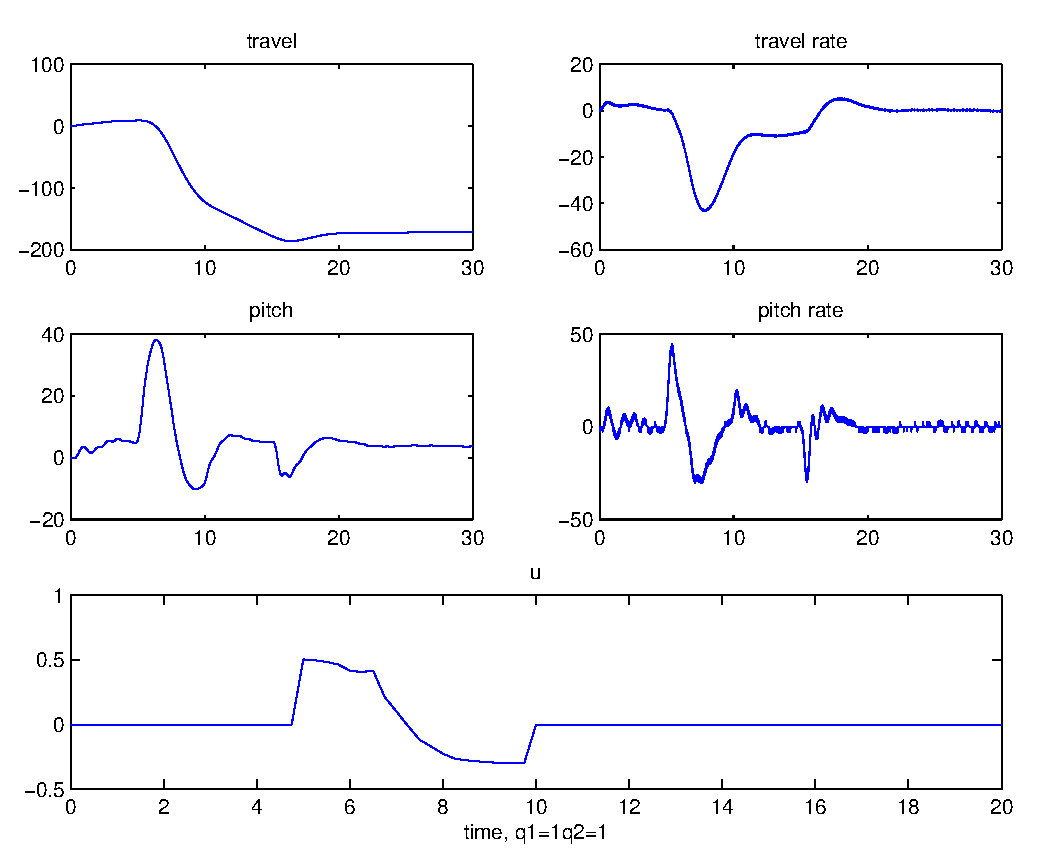
\includegraphics[scale=0.8]{{figures/10.4.3.q1_1_q2_1_N_40}.eps}
\caption{Closed loop response in of the system for case 10.4 (N=40)}
\label{fig:feedback-4-closed}
\end{figure}

\begin{figure}[H]
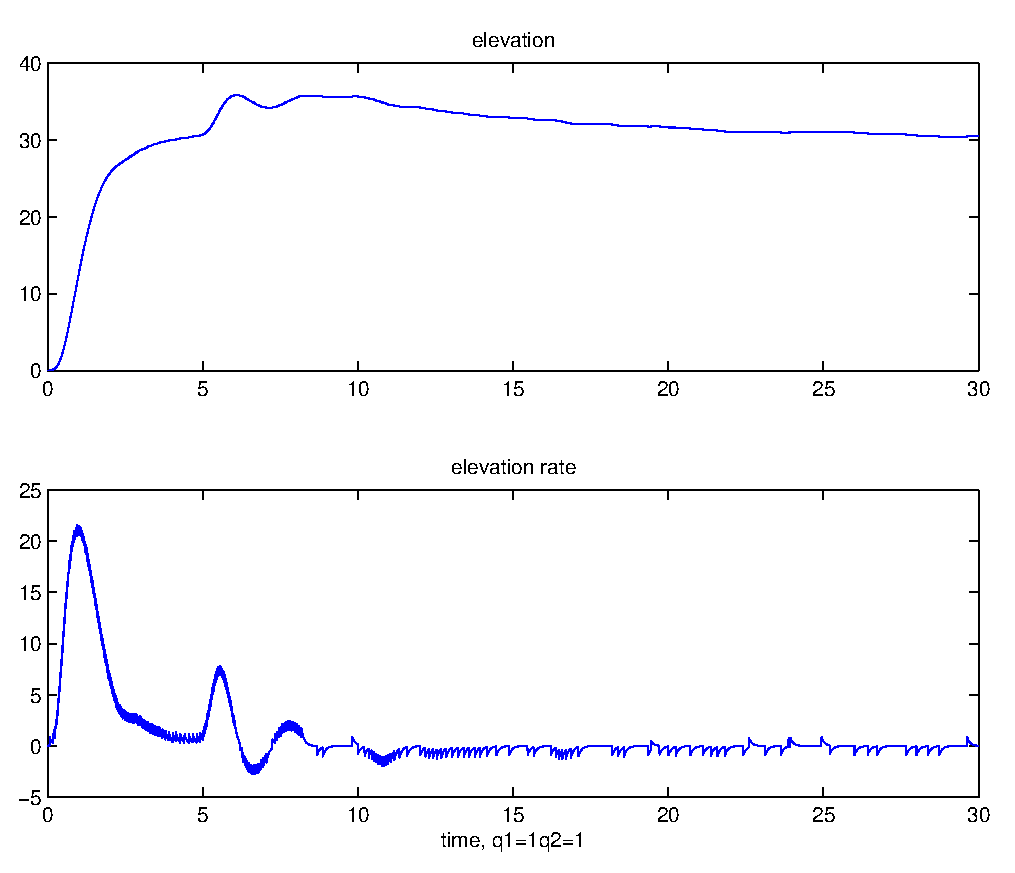
\includegraphics[scale=0.8]{{figures/10.4.3.elevation.q1_1_q2_1_N_40}.eps}
\caption{Closed loop elevation of the system for case 10.4 (N=40)}
\label{fig:feedback-4-closed-elevation}
\end{figure}

\begin{figure}[H]
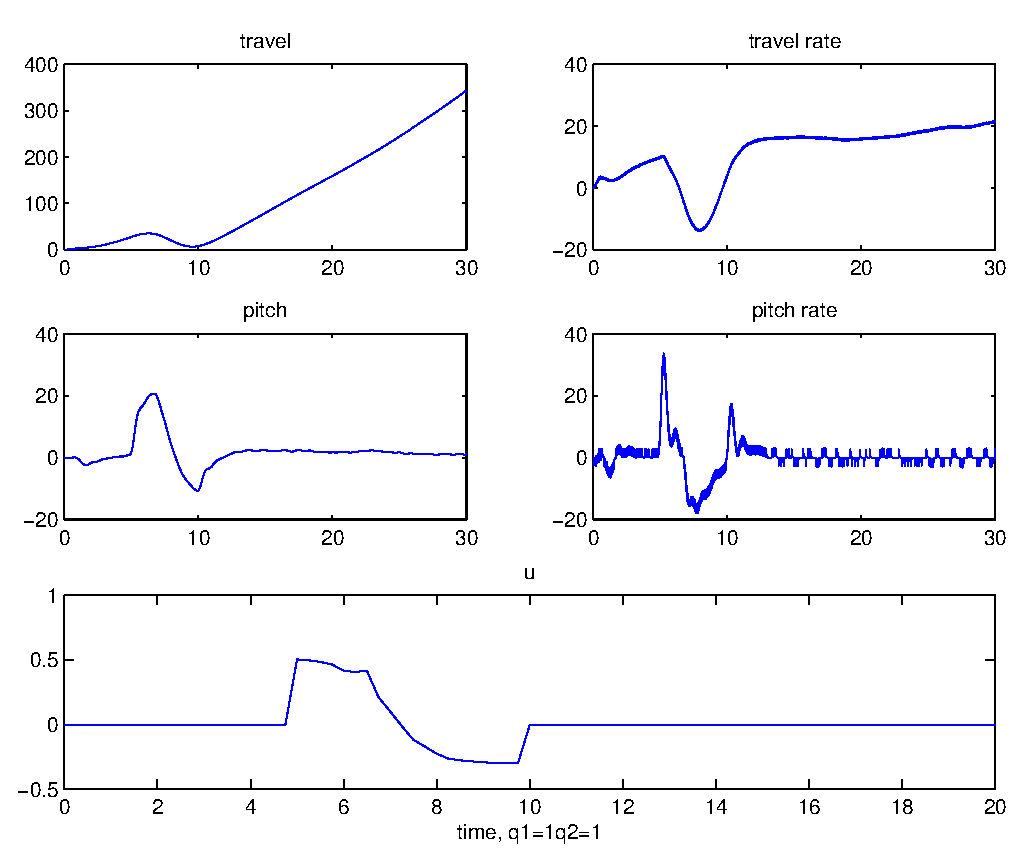
\includegraphics[scale=0.8]{{figures/openloop10.4.3.q1_1_q2_1_N_40}.eps}
\caption{Open loop response in of the system for case 10.4 (N=40)}
\label{fig:feedback-4-open}
\end{figure}

\begin{figure}[H]
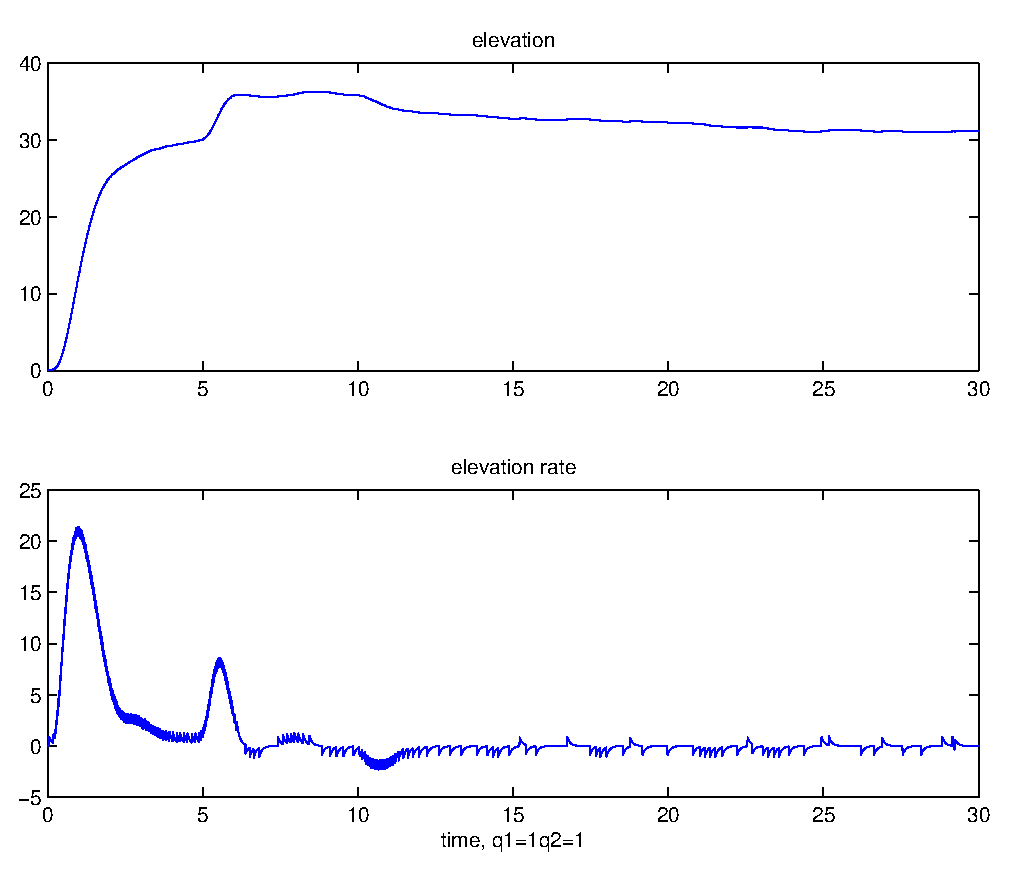
\includegraphics[scale=0.8]{{figures/openloop10.4.3.elevation.q1_1_q2_1_N_40}.eps}
\caption{Open loop elevation of the system for case 10.4 (N=40)}
\label{fig:feedback-4-open-elevation}
\end{figure}


\subsubsection{Decoupled States}
% Notice that the first 4 states in the model are completely decoupled from the last 2. How does this fit with reality? What effect does this have on the calculated optimal trajectory? Suggest [but do not implement] a solution to improve this.
The decoupled stats do not seem to conform to reality, as a pitch would affect any elevation inputs which will increase the speed in which the pitch is pointing, affecting the optimal trajectory such that it isn't able to completely conform to it using the calculated $u*$. The solution would be to formulate a nonlinear system and linearize it at each point so that it can be controlled using conventional methods.

\subsubsection{Adding More Constraints}
% Optional exercise: Try adding more constraints on the states. These ̇may be constraints on maximal allowed speed e  ̇ and λ.
One constraint to add is to state that the second element of $xl$ and $xu$ to about $0.1$, which was implemented in \Cref{lst:problem_4}. This made the helicopter turn very slowly (about 6 degrees per second), however, its elevation became more easily noticable.

\section{Results and Figures}\label{sec:figures}
Answer all the parts of the exercise in an organized and clear manner. You should of course try to get good results in all the exercises, but if you have made a good effort without achieving great performance, a good discussion of possible reasons is just as good. Present your thinking and efforts and discuss possible reasons for good or bad results.

Include plots and/or tables of all relevant results, but make sure you don't overwhelm the reader with too many plots. Have a clear plan about what you want to communicate with a specific plot/figure, and use appropriate labels and comments. Keep in mind that the plots should be as ``readable'' as possible; that is, they should not be too hard to interpret and be reasonably self contained.

There are some important things to consider when exporting figures from MATLAB, most importantly which format you use. Never ever use JPEG for anything that is not a photography or similar. Any figure, like a plot or block diagram, must never be stored as a JPEG\@. If you zoom in on \Cref{fig:constraint_jpg} you can see a lot of noise close to any of the dark curves and lines, this is due to the compression in JPEG\@. \Cref{fig:constraint_jpg} will look horrible both on a screen and on paper.

The PNG format is slightly better for plots, but since it is a raster format (a grid of pixels), it looks ugly if you zoom in. It also looks ugly if you scale it, both on a screen and on paper. Try to avoid PNG if you can. \Cref{fig:constraint_png,fig:constraint_png_large} are both PNG figures; the latter being a larger figure scaled more than the former. Note both how choppy and ugly the blue curve is, and how the different sizes create inconsistent font sizes.

The simplest way to get a reasonably good looking plot is to save it as EPS in MATLAB\@. Do this by clicking ``File'' in the figure window, and the ``Save As\ldots''; choose ``EPS file (*.eps)'' in the ``Save as type:'' menu.\footnote{pdfLatex does not support EPS directly, but since we have loaded the \emph{epstodf} package, this is not a problem.} \Cref{fig:constraint_eps} shows a plot in EPS format. Since EPS is a vector format, the Figure can be scaled and still look good (but mind the font size!). If you zoom in you can see that the curve and the letters/numbers are smooth. A figure in vector format will usually look good both on a screen and on paper.

Note that the size of the actual figure window in MATLAB determines how large the exported figure is. Hence, if you enlarge the figure window before exporting, you will need to scale the figure by a larger factor in the report. This will lead to a tiny font in the figure. There are many better ways of exporting graphics from MATLAB, but they quickly become fairly involved. The above method of exporting to EPS will in most cases give nice figures.

You can write Latex in your MATLAB figures. The script used to create \Cref{fig:constraint_jpg,fig:constraint_eps} is included in \Cref{sec:plot_constraint_m}. Do not use a screen shot of a scope of figure in MATLAB in your report.

\begin{figure}[htb]
	\centering
		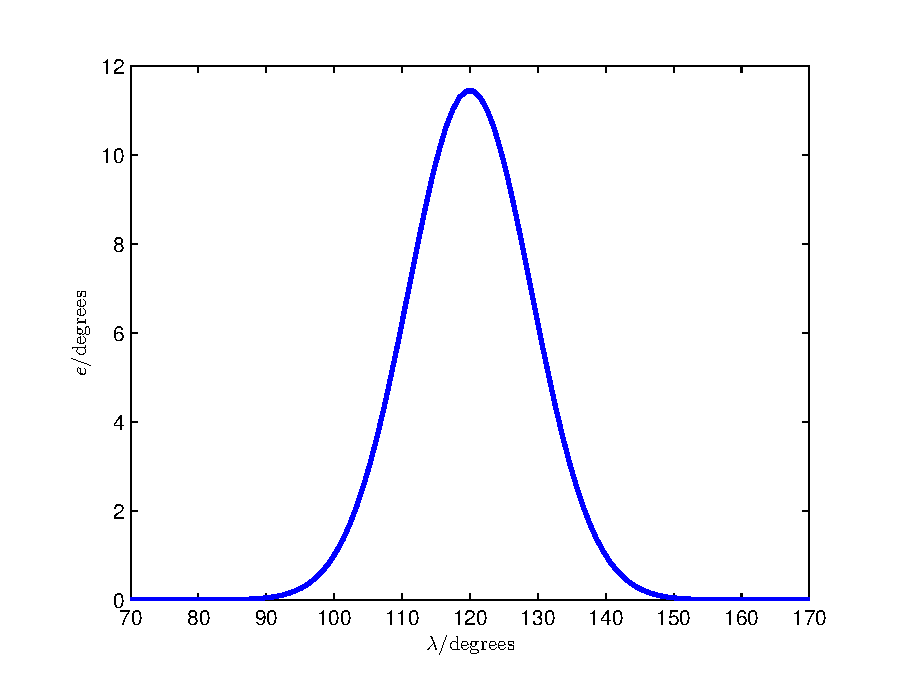
\includegraphics[width=0.8\textwidth]{figures/constraint_eps.eps}
	\caption{A plot in EPS format --- a much better idea.}
\label{fig:constraint_eps}
\end{figure}

Remember to reference all figures in the text. Figures have a number and should be referenced by that number (again, always use dynamic references). They also tend to float around, meaning they generally don't appear where you ask them to in the text. This is fine, do not try to force a figure (or a table) to appear in a particular place. As long a you refer to it, it's easy to find. No figure should be included without being referenced in the text.

If you look at the source code for including figures, you can see that the optional option \verb+[htb]+ has been used. This tells Latex where you wish the figure to appear, in prioritized order. \verb+h+ means ``Here'', t means ``Top of this page'', b means ``Bottom of this page'', and p (not used here) means ``on a Page with only floats (such as figures and tables)''. Note that your wish might not be granted, and this is because Latex actually optimizes the placement of figures. If you start forcing figures to be in specific places, it often leads to really strange layout somewhere else in the document.

Generally, let Latex handle the documentation layout. This is one of the main reasons to choose Latex over software such as Microsoft Word.

\subsection{Results and Discussion}
All problems should have their own discussion of results.

Remember: all plots and results need a description, explanation, and discussion.

\section{Conclusion}\label{sec:conclusion}
This does not have to be long, but try to write a few reasonable closing remarks.

\addcontentsline{toc}{section}{Appendix} % Remove this if you don't want the appendix included in the table of contents.
\appendix

\section{MATLAB Code}\label{sec:matlab}
This section documents our MATLAB code.

\subsection{problem\_2.m}
\lstinputlisting[language=Matlab,caption={Problem 2 code},label=lst:problem_2]{../problem_2.m}
\subsection{compute\_lq.m}
\lstinputlisting[language=Matlab,caption={Script for computing the LQ k gain},label=lst:compute_lq]{../compute_lq.m}

\subsection{problem\_3.m}
\lstinputlisting[language=Matlab,caption={Problem 3 code},label=lst:problem_3]{../problem_3.m}
\subsection{problem\_4.m}
\lstinputlisting[language=Matlab,caption={Problem 4 code},label=lst:problem_4]{../problem_4.m}
\subsection{nonlcon.m}
\lstinputlisting[language=Matlab,caption={Nonlinear constraint function},label=lst:nonlcon]{../nonlcon.m}
\subsection{compute\_lq4.m}
\lstinputlisting[language=Matlab,caption={Compute LQ for the fourth problem},label=lst:compute_lq4]{../compute_lq4.m}

\subsection{plot2s3.m}
\lstinputlisting[language=Matlab,caption={Plot the test run for case 10.2},label=lst:plot2s3]{../plot2s3.m}
\subsection{plot3s3.m}
\lstinputlisting[language=Matlab,caption={Plot the test run for case 10.3},label=lst:plot3s3]{../plot3s3.m}
\subsection{plot4s3.m}
\lstinputlisting[language=Matlab,caption={Plot the test run for case 10.4},label=lst:plot4s3]{../plot4s3.m}

\section{Simulink Diagrams}\label{sec:simulink}
This section contains Simulink diagrams.

\subsection{No Feedback}
\begin{figure}[H]
	\centering
		\includegraphics[scale=0.3]{figures/{2-simulinksim_helicopter}.eps}
	\caption{The simulink model used for optimal open loop control.}
\label{fig:2-simulink}
\end{figure}

\subsection{Feedback (LQ)}
\begin{figure}[H]
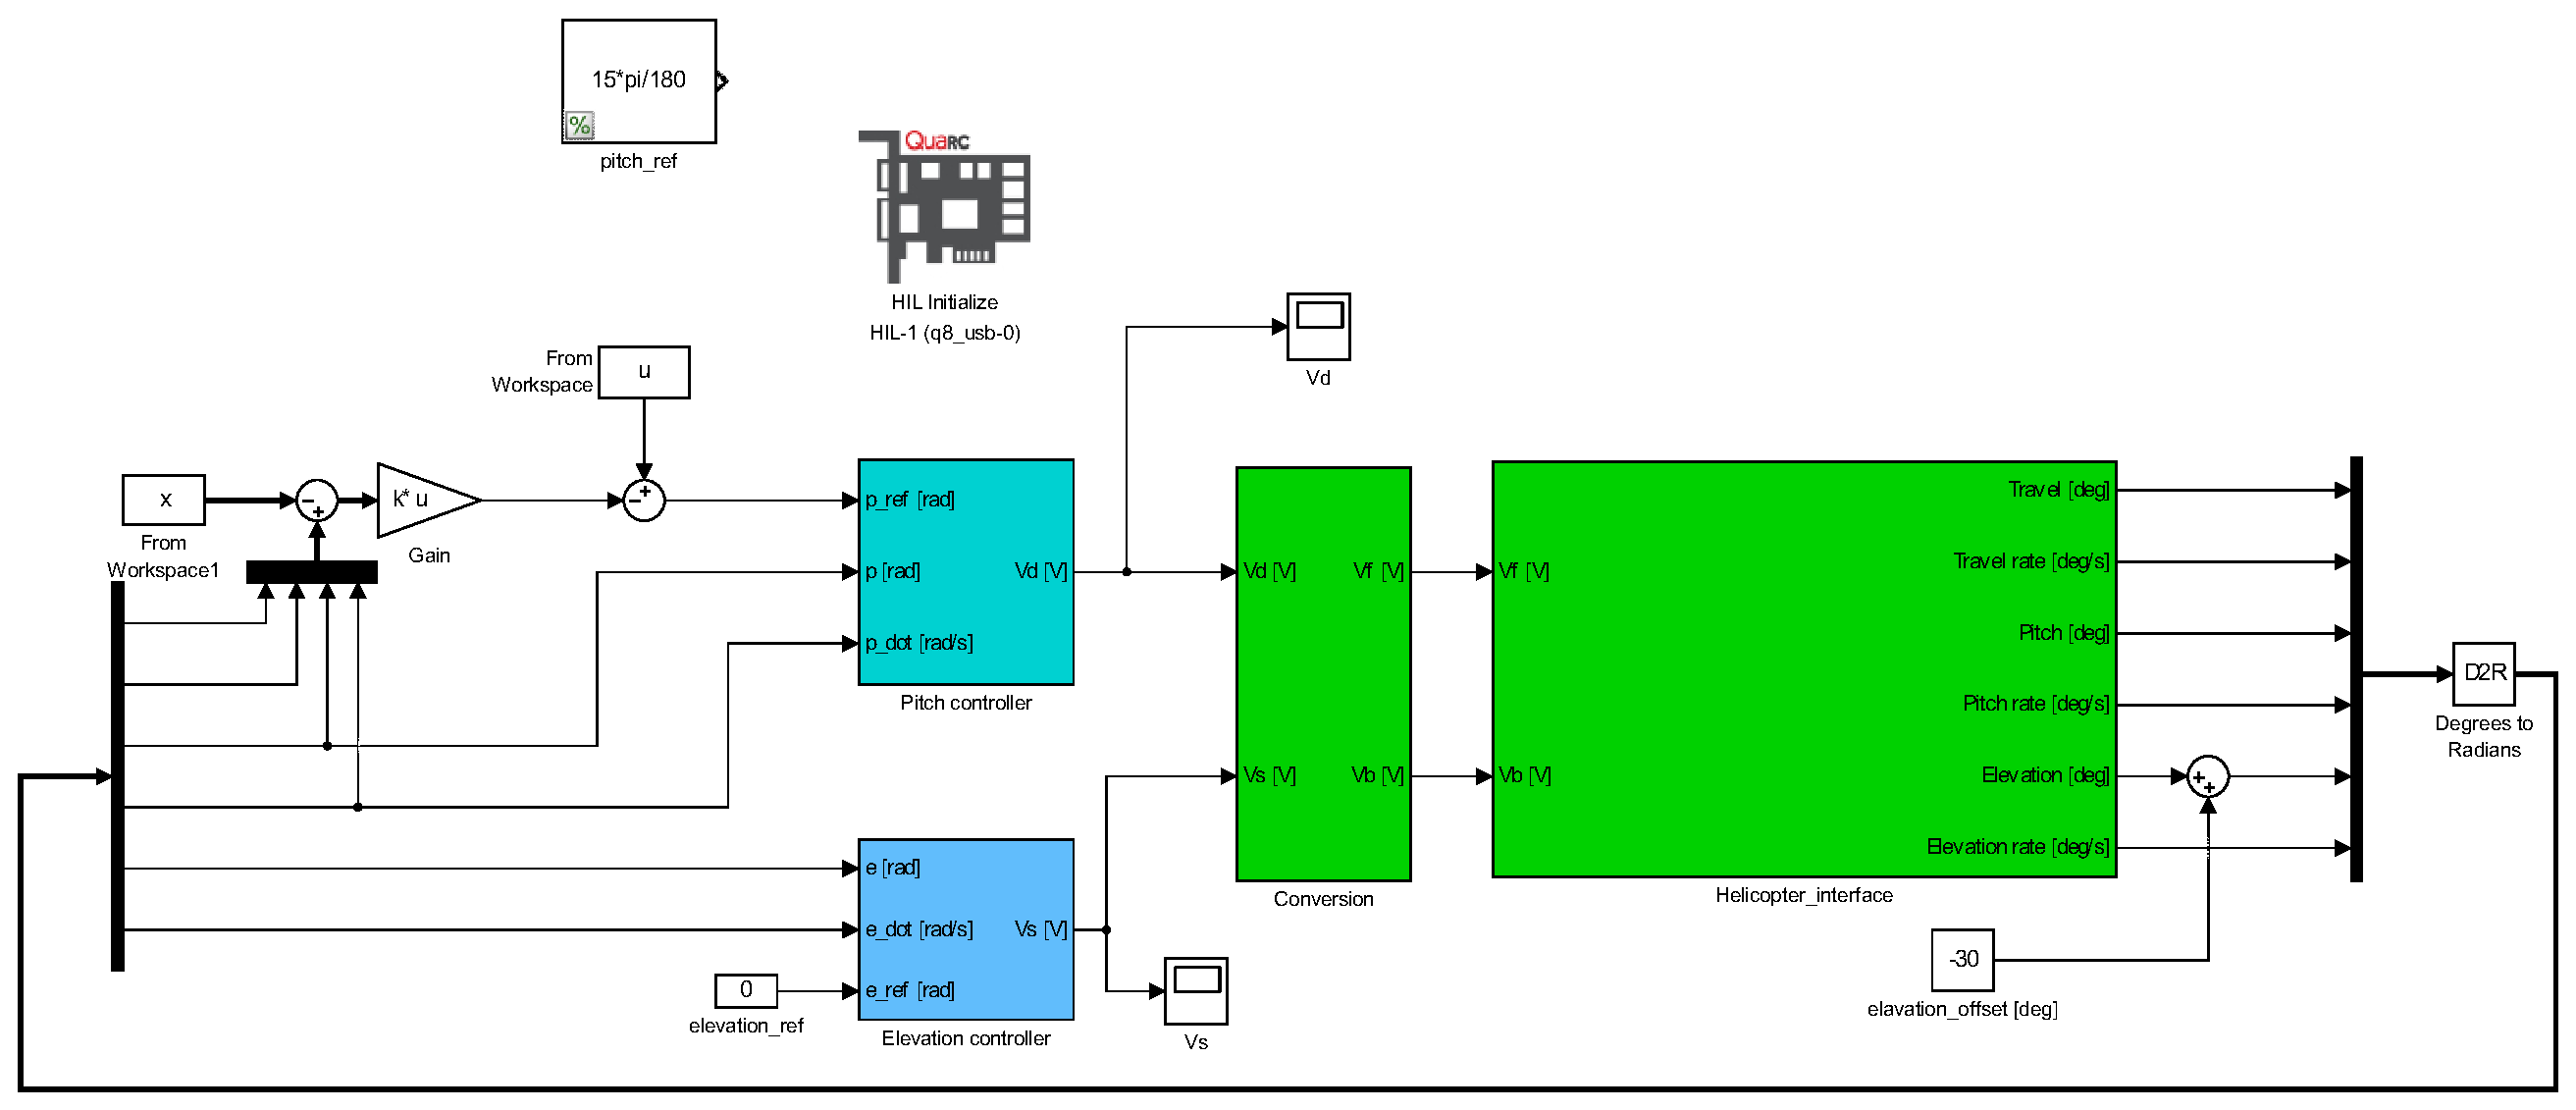
\includegraphics[scale=0.3]{figures/3-simulinksim_helicopter.eps}
\caption{Feedback system for the helicopter with static elevation control}
\label{fig:feedback-3}
\end{figure}

\subsection{Pitch and Elevation Control}
\begin{figure}[H]
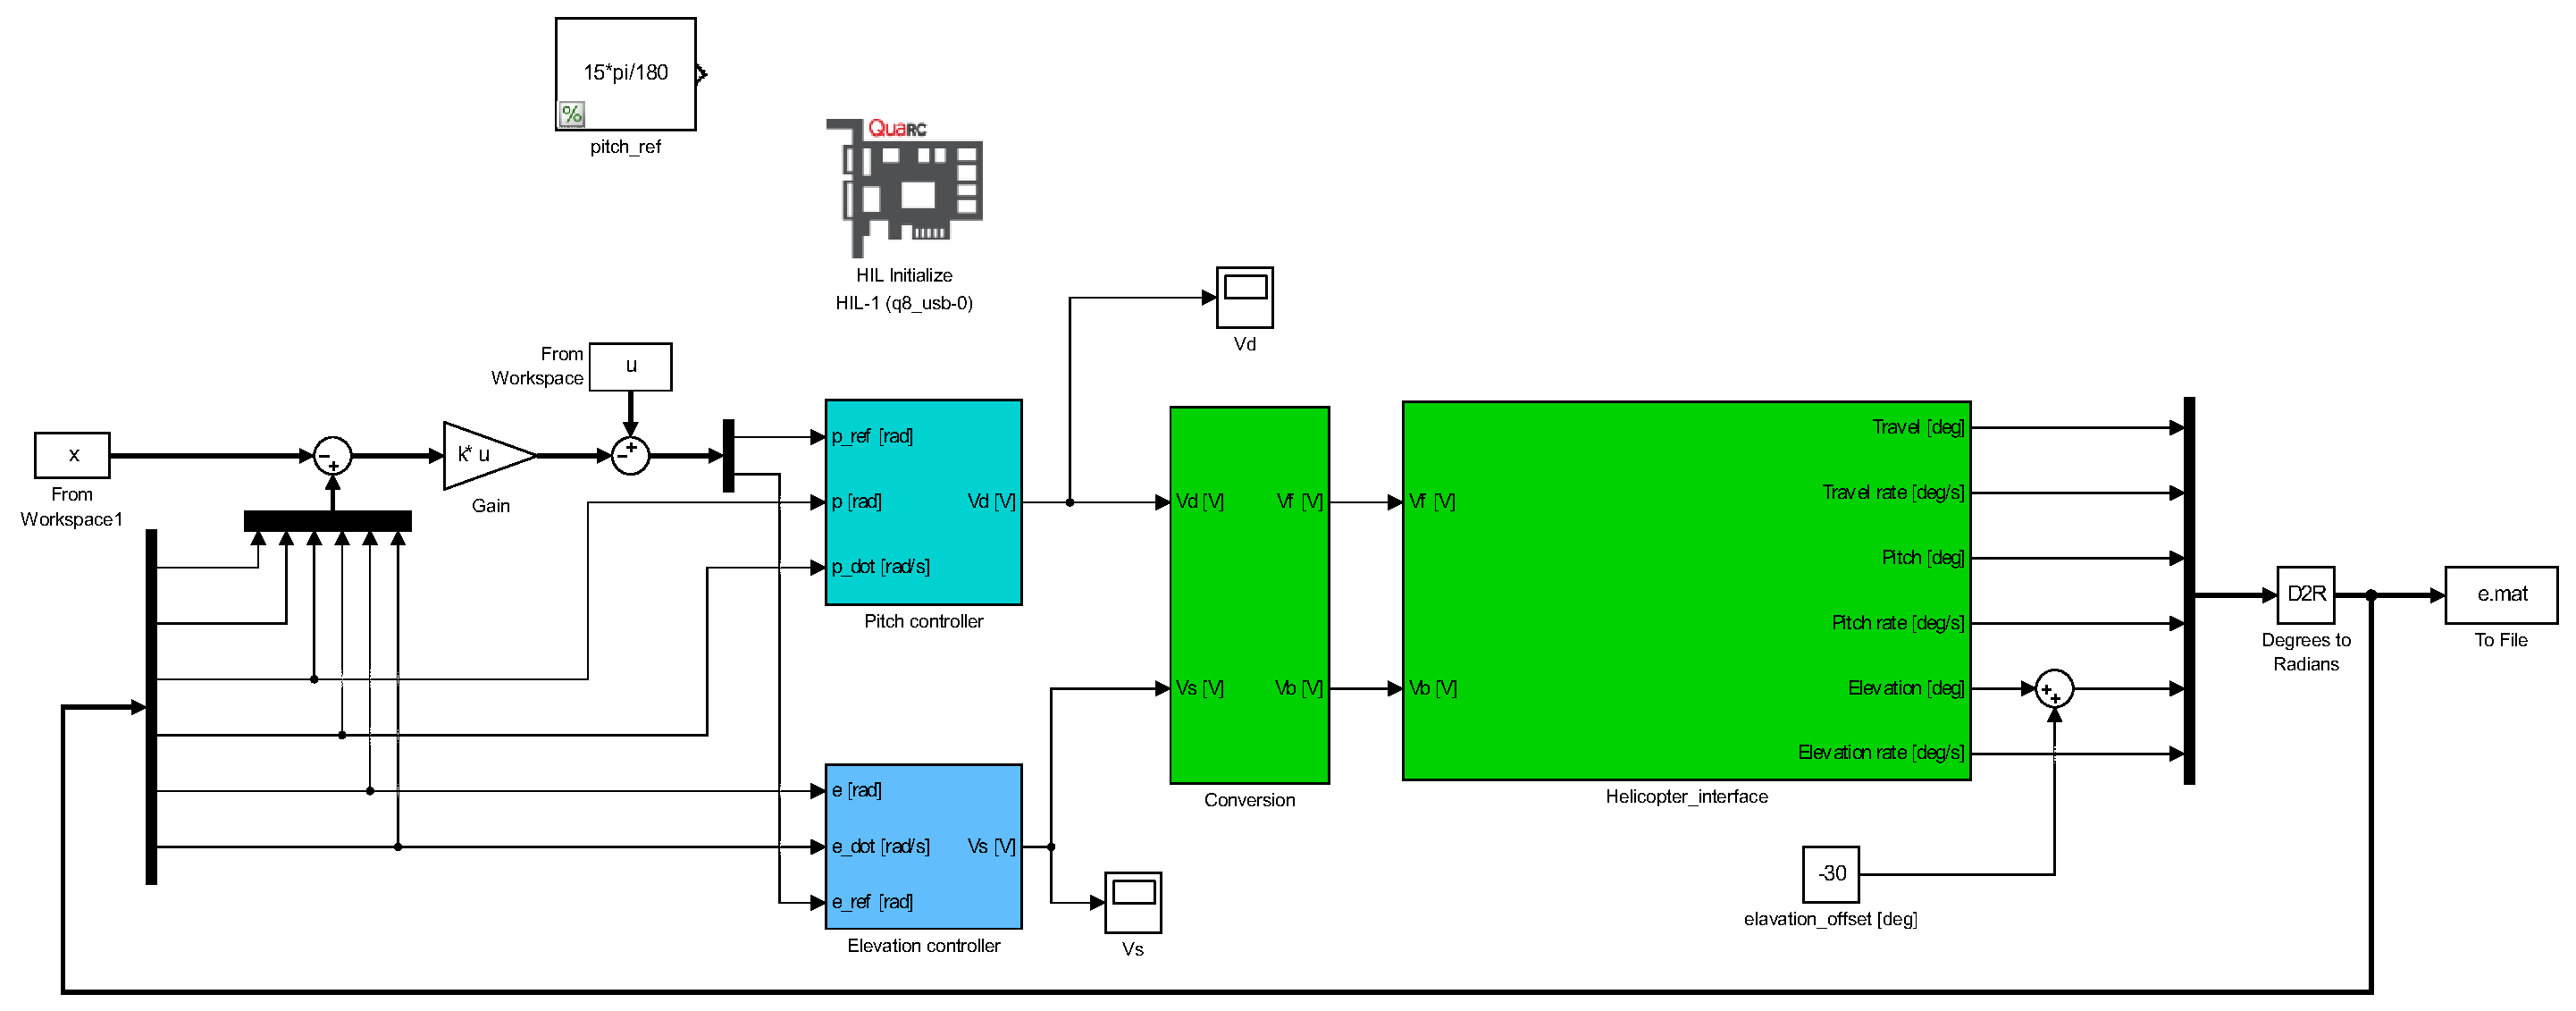
\includegraphics[scale=0.3]{{figures/4-simulinksim_helicopter}.eps}
\caption{Feedback system for the helicopter (N=40), for the non-feedback case the constant gain is zerod.}
\label{fig:feedback-4}
\end{figure}

\section{Lab exercises}\label{sec:ex}

\includepdf[pages={-}]{LabExercise.pdf}


% \input simply inserts the contents of the file, while \include forces a \newpage.
% See \input vs. \include: http://tex.stackexchange.com/questions/246/when-should-i-use-input-vs-include

% References
\newpage
\addcontentsline{toc}{section}{References}
\printbibliography{}
\label{sec:bibliography}

\end{document}
